\documentclass{beamer}
\mode<presentation>
\usepackage[orientation=portrait,size=a0,scale=1.4]{beamerposter}
\usetheme{gemini}
\usecolortheme{gemini}
\usepackage{siunitx}
\usepackage{wrapfig}
\usepackage{natbib}
\usepackage{floatrow}

\usepackage{filecontents}
\begin{filecontents*}{\jobname.bib}
    @article{posen2021advances,
        title={Advances in Nb\textsubscript{3}Sn superconducting radiofrequency cavities towards first practical accelerator applications},
        author={Posen, Sam and Lee, Jaeyel and Seidman, David N and Romanenko, Alexander and Tennis, Brad and Melnychuk, OS and Sergatskov, DA},
        journal={Superconductor Science and Technology},
        volume={34},
        number={2},
        pages={025007},
        year={2021},
        publisher={IOP Publishing}
    }   
\end{filecontents*}

\setbeamertemplate{bibliography entry article}{}
\setbeamertemplate{bibliography entry title}{}
\setbeamertemplate{bibliography entry location}{}
\setbeamertemplate{bibliography entry note}{}


\title{Improving Nb\textsubscript{3}Sn Cavity Performance Using Mechanical Polishing}%
\author{Eric Viklund \inst{1, 2} \and David Burk \inst{2} \and David N. Seidman \inst{1} \and Sam Posen \inst{2}}
\institute[shortinst]{\inst{1} Department of Materials Science and Engineering, Northwestern University \samelineand \inst{2} Fermi National Accelerator Laboratory}
\date{\today}%

\logoleft{\parbox{0.05\textwidth}{
\includegraphics[width=7cm]{logos/FNAL-Logo-White.png} 
\includegraphics[width=7cm]{logos/Northwestern-Logo-White.png}}}

\begin{document}%
    \begin{frame}{}
        %\maketitle
        \begin{columns}[t]
            \begin{column}{0.32\linewidth}
                \begin{alertblock}{\label{sec:introduction}Key Findings}
                    \begin{itemize}
                        \item Centrifugal barrel polishing (CBP) is an effective method of polishing Nb\textsubscript{3}Sn coated cavities.
                        \item Nb\textsubscript{3}Sn films polished using CBP can acheive less than 20~nm surface roughness with minimal material removal.
                        \item CBP treatment of a Nb\textsubscript{3}Sn cavity leads to a significant increase in the maximum accelerating gradient.
                        \item However, a secondary re-coating procedure is required to achive this increase.
                    \end{itemize}
                \end{alertblock}
                \begin{block}{\label{sec:backgroundinformation}Background Information}
                    Superconducting radiofrequency (SRF) cavities are essential components for providing the electric fields required to accelerate charged particles in particle accelerators. SRF cavities coated with a layer of Nb\textsubscript{3}Sn can reach up to 100~MV/m of accelerating field in theory. However, in practice surface roughness and other defects limit Nb\textsubscript{3}Sn SRF cavity performance. Centrifugal barrel polishing (CBP) is a proven technique for mechanically polishing Nb SRF cavities to nanometer scale smoothness. To show the evolution of the surface during CBP, we polish Nb\textsubscript{3}Sn samples using a coupon cavity, which can simulate cavity polishing conditions.
                    \begin{columns}[t]
                        \begin{column}{0.45\columnwidth}
                            \begin{itemize}
                                \item Centrifugal Barrel Polishing (CBP) is a technique used to polish niobium cavities without using toxic chemicals such as HF.
                                \item CBP uses a custom built tumbling machine that can fit up to 9-cell size cavities, and can accelerate the polishing media against the cavity surface with up to 6g of force.
                                \item An alumina nanoparticle suspension is used as the abrasive material. Felt cubes are added to push the abrasives against the cavity surface.
                            \end{itemize}  
                        \end{column}
                        \begin{column}{0.45\columnwidth}
                            \begin{figure}[t]%
                                \centering%
                                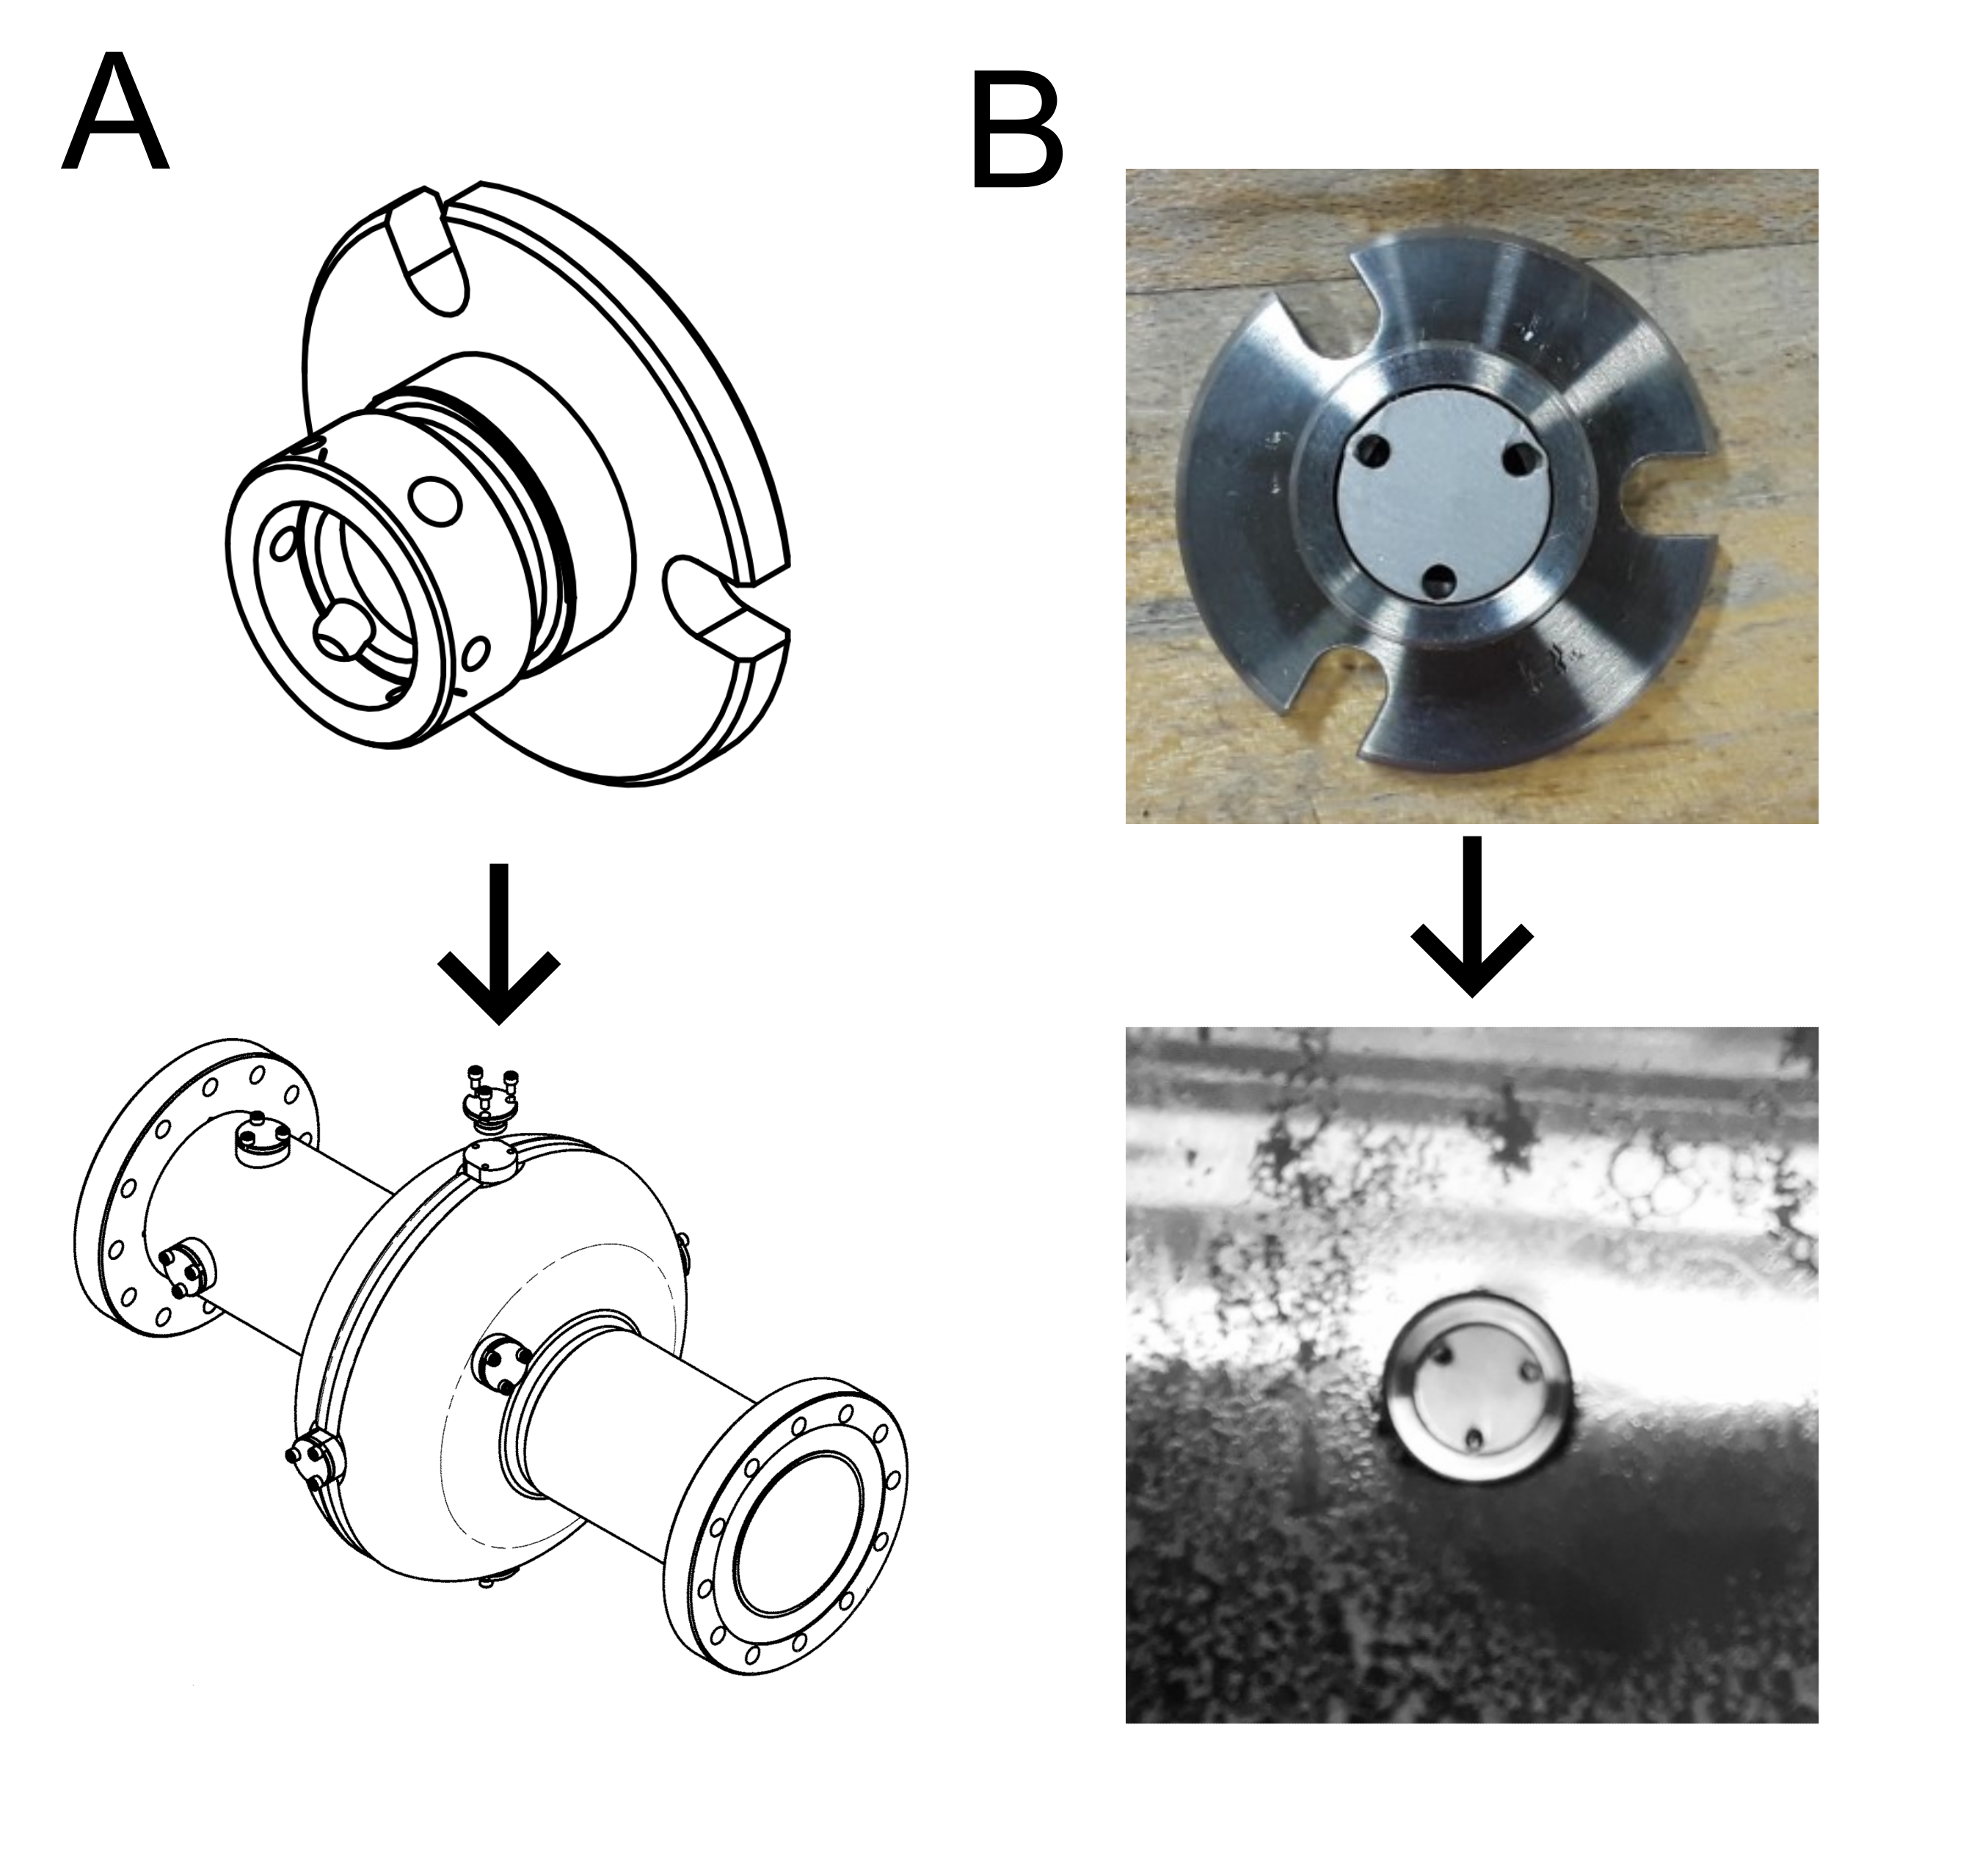
\includegraphics[width=\columnwidth]{../doc/figs/Coupon_Cavity.png}%
                                \caption{(A) A schematic of the coupon cavity and the sample holder used to polish the Nb\textsubscript{3}Sn coated samples. The sample holder can hold 1~cm diameter disks by clamping the sides of the sample with set screws. (B) Pictures of the sample holder sitting outside the coupon cavity and with a sample mounted as seen from the inside of the coupon cavity.}%
                                \label{fig:couponcavity}%
                            \end{figure}
                        \end{column}
                    \end{columns}
                \end{block}
            \end{column}





            \begin{column}{0.32\linewidth}    
                \begin{block}{\label{sec:samplestudy}Surface Analysis of Nb\textsubscript{3}Sn Polished with CBP}
                    \begin{columns}[t]
                        \begin{column}{0.4\columnwidth}
                            \begin{figure}[t]
                                \centering
                                \includegraphics[width=\columnwidth]{../doc/figs/Optical_Surface_Profiles.png}
                                \caption{\label{fig:opticalsurfaceprofiles}Surface height maps of Nb\textsubscript{3}Sn polished between 0 to 8~hours.}
                            \end{figure}

                        \end{column}
                        \begin{column}{0.5\columnwidth}
                             \begin{figure}[t]
                                \centering
                                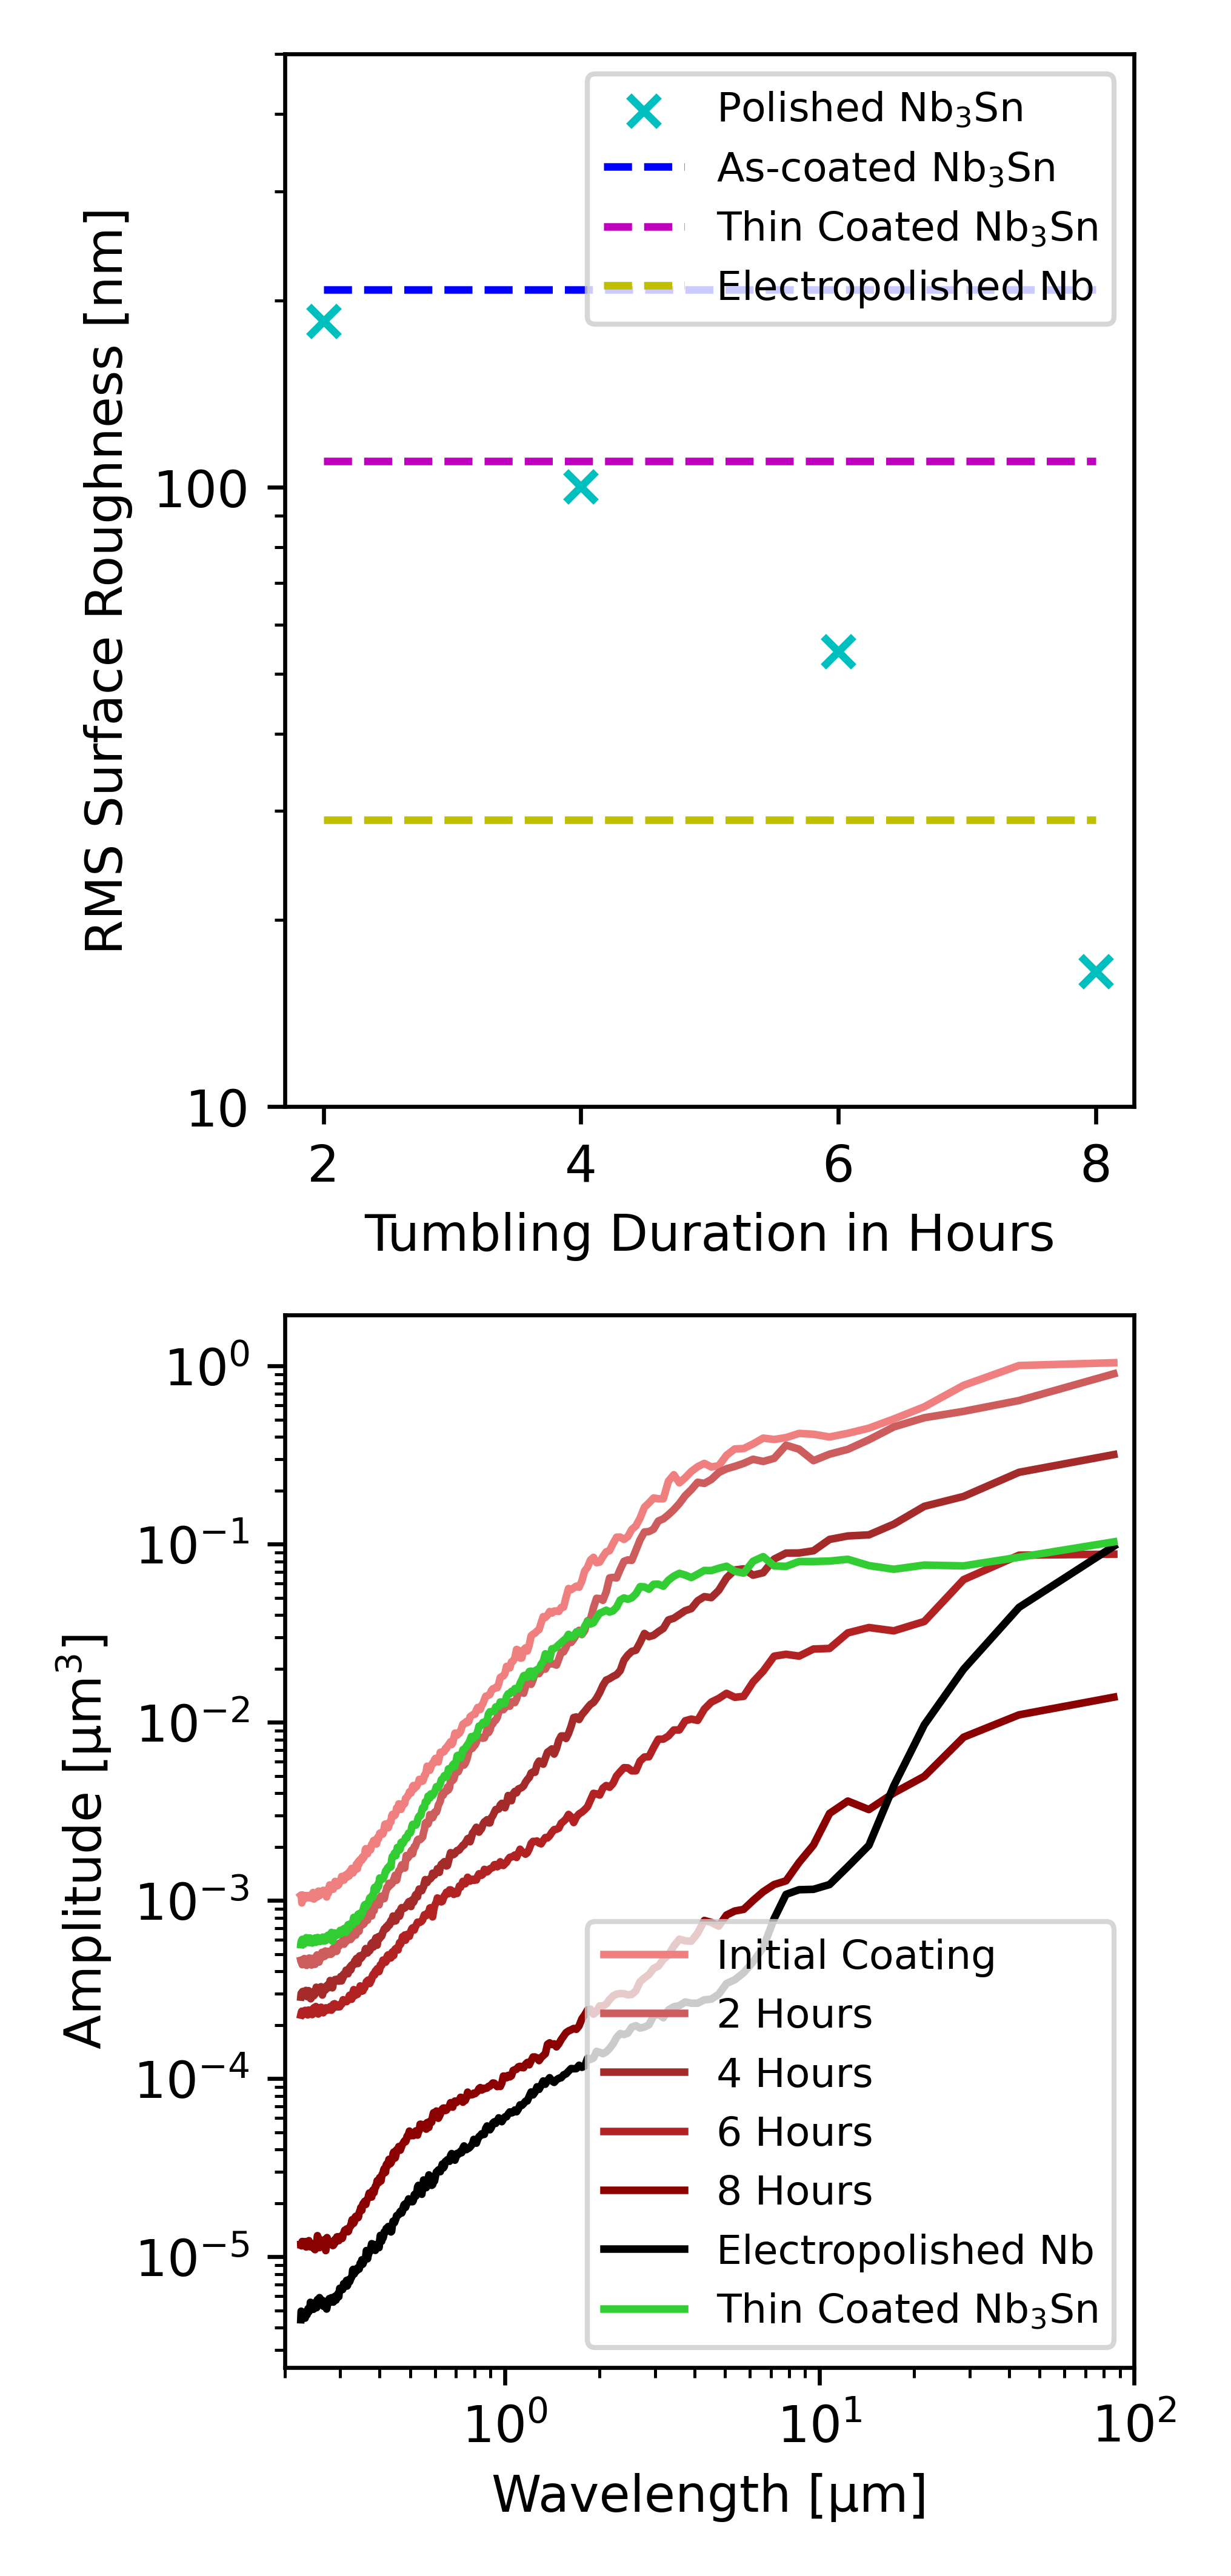
\includegraphics[width=\columnwidth]{../doc/figs/Surface_Roughness_Graph.png}
                                \caption{\label{fig:surfaceroughnessgraph}Surface roughness of Nb\textsubscript{3}Sn over time (top). The power spectral density (PSD) of the surface profiles, electropolished Nb, and thinly coated Nb\textsubscript{3}Sn\cite{posen2021advances}.}
                            \end{figure}
                        \end{column}

                    \end{columns}
                    To evaluate the performance of CBP, the surface roughness of the polished samples is measured using con-focal laser microscopy and the surface is analyzed using scanning and transmission electron microscopy (SEM and TEM). The material removal rate is measured using focused ion-beam tomography.
                    \begin{itemize}                        
                        \item Material is preferentially removed from the highest point on the surface.
                        \item The material removal rate is measured to be 170~nm per hour.
                        \item After 6~hours of polishing, the surface roughness is comparable to the surface roughness of the well-performing, thinly coated Nb\textsubscript{3}Sn coatings created at Fermilab\cite{posen2021advances}.
                        \item After 8~hours of polishing, the surface roughness is comparable to a typical niobium surface after EP.
                    \end{itemize}
                    \begin{figure}
                        \floatbox[{\capbeside\thisfloatsetup{capbesideposition={left,top},capbesidewidth=4cm}}]{figure}[\FBwidth]
                        {\caption{TEM images of a Nb\textsubscript{3}Sn sample polished using wooden spheres (A) and felt cubes (B). The polishing procedure creates a 10~nm thick layer of disordered Nb\textsubscript{3}Sn on the sample polished with wooden spheres which is not present on the sample polished by felt cubes.}\label{fig:samplesurfacedamagelayer}}
                        {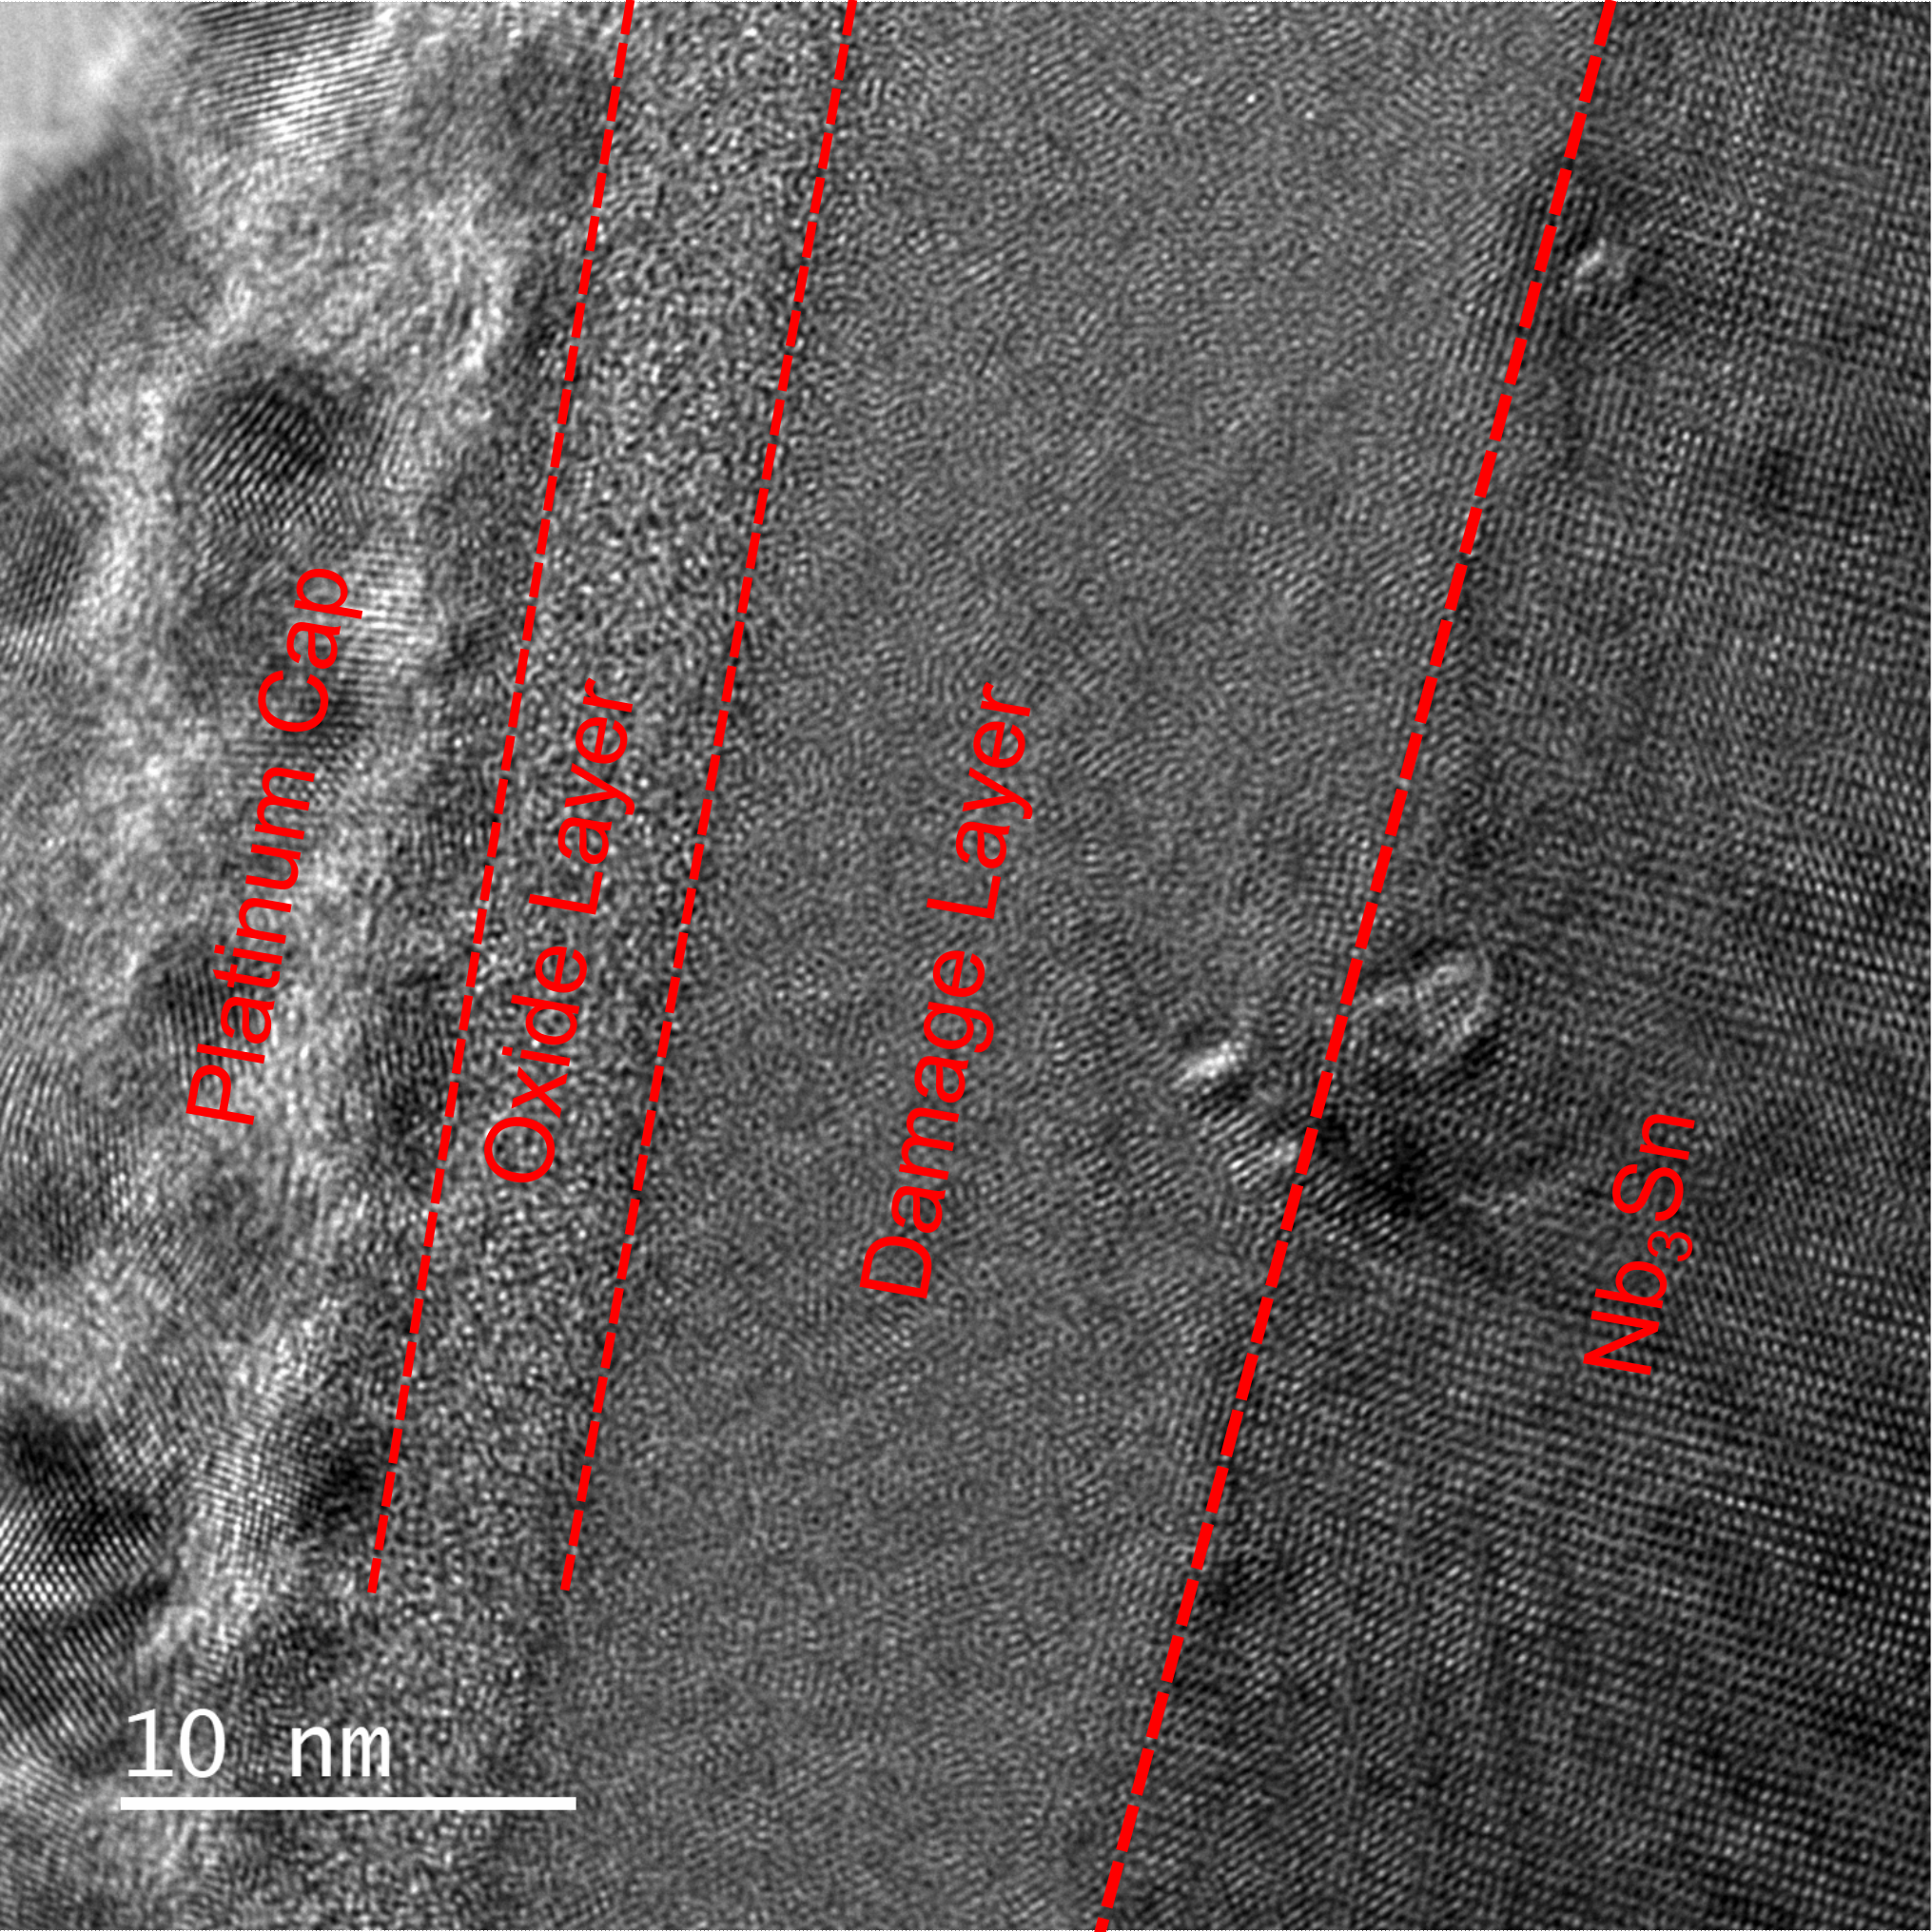
\includegraphics[width=\columnwidth]{../doc/figs/Sample_Surface_Damage_Layer.png}}
                    \end{figure}

                \end{block}
            \end{column}





            \begin{column}{0.32\textwidth}
                \begin{block}{\label{sec:cavitycbp}RF Performance Improvement from Polishing}
                    \begin{columns}
                        \begin{column}{0.45\columnwidth}
                            \begin{figure}[t]
                                \centering
                                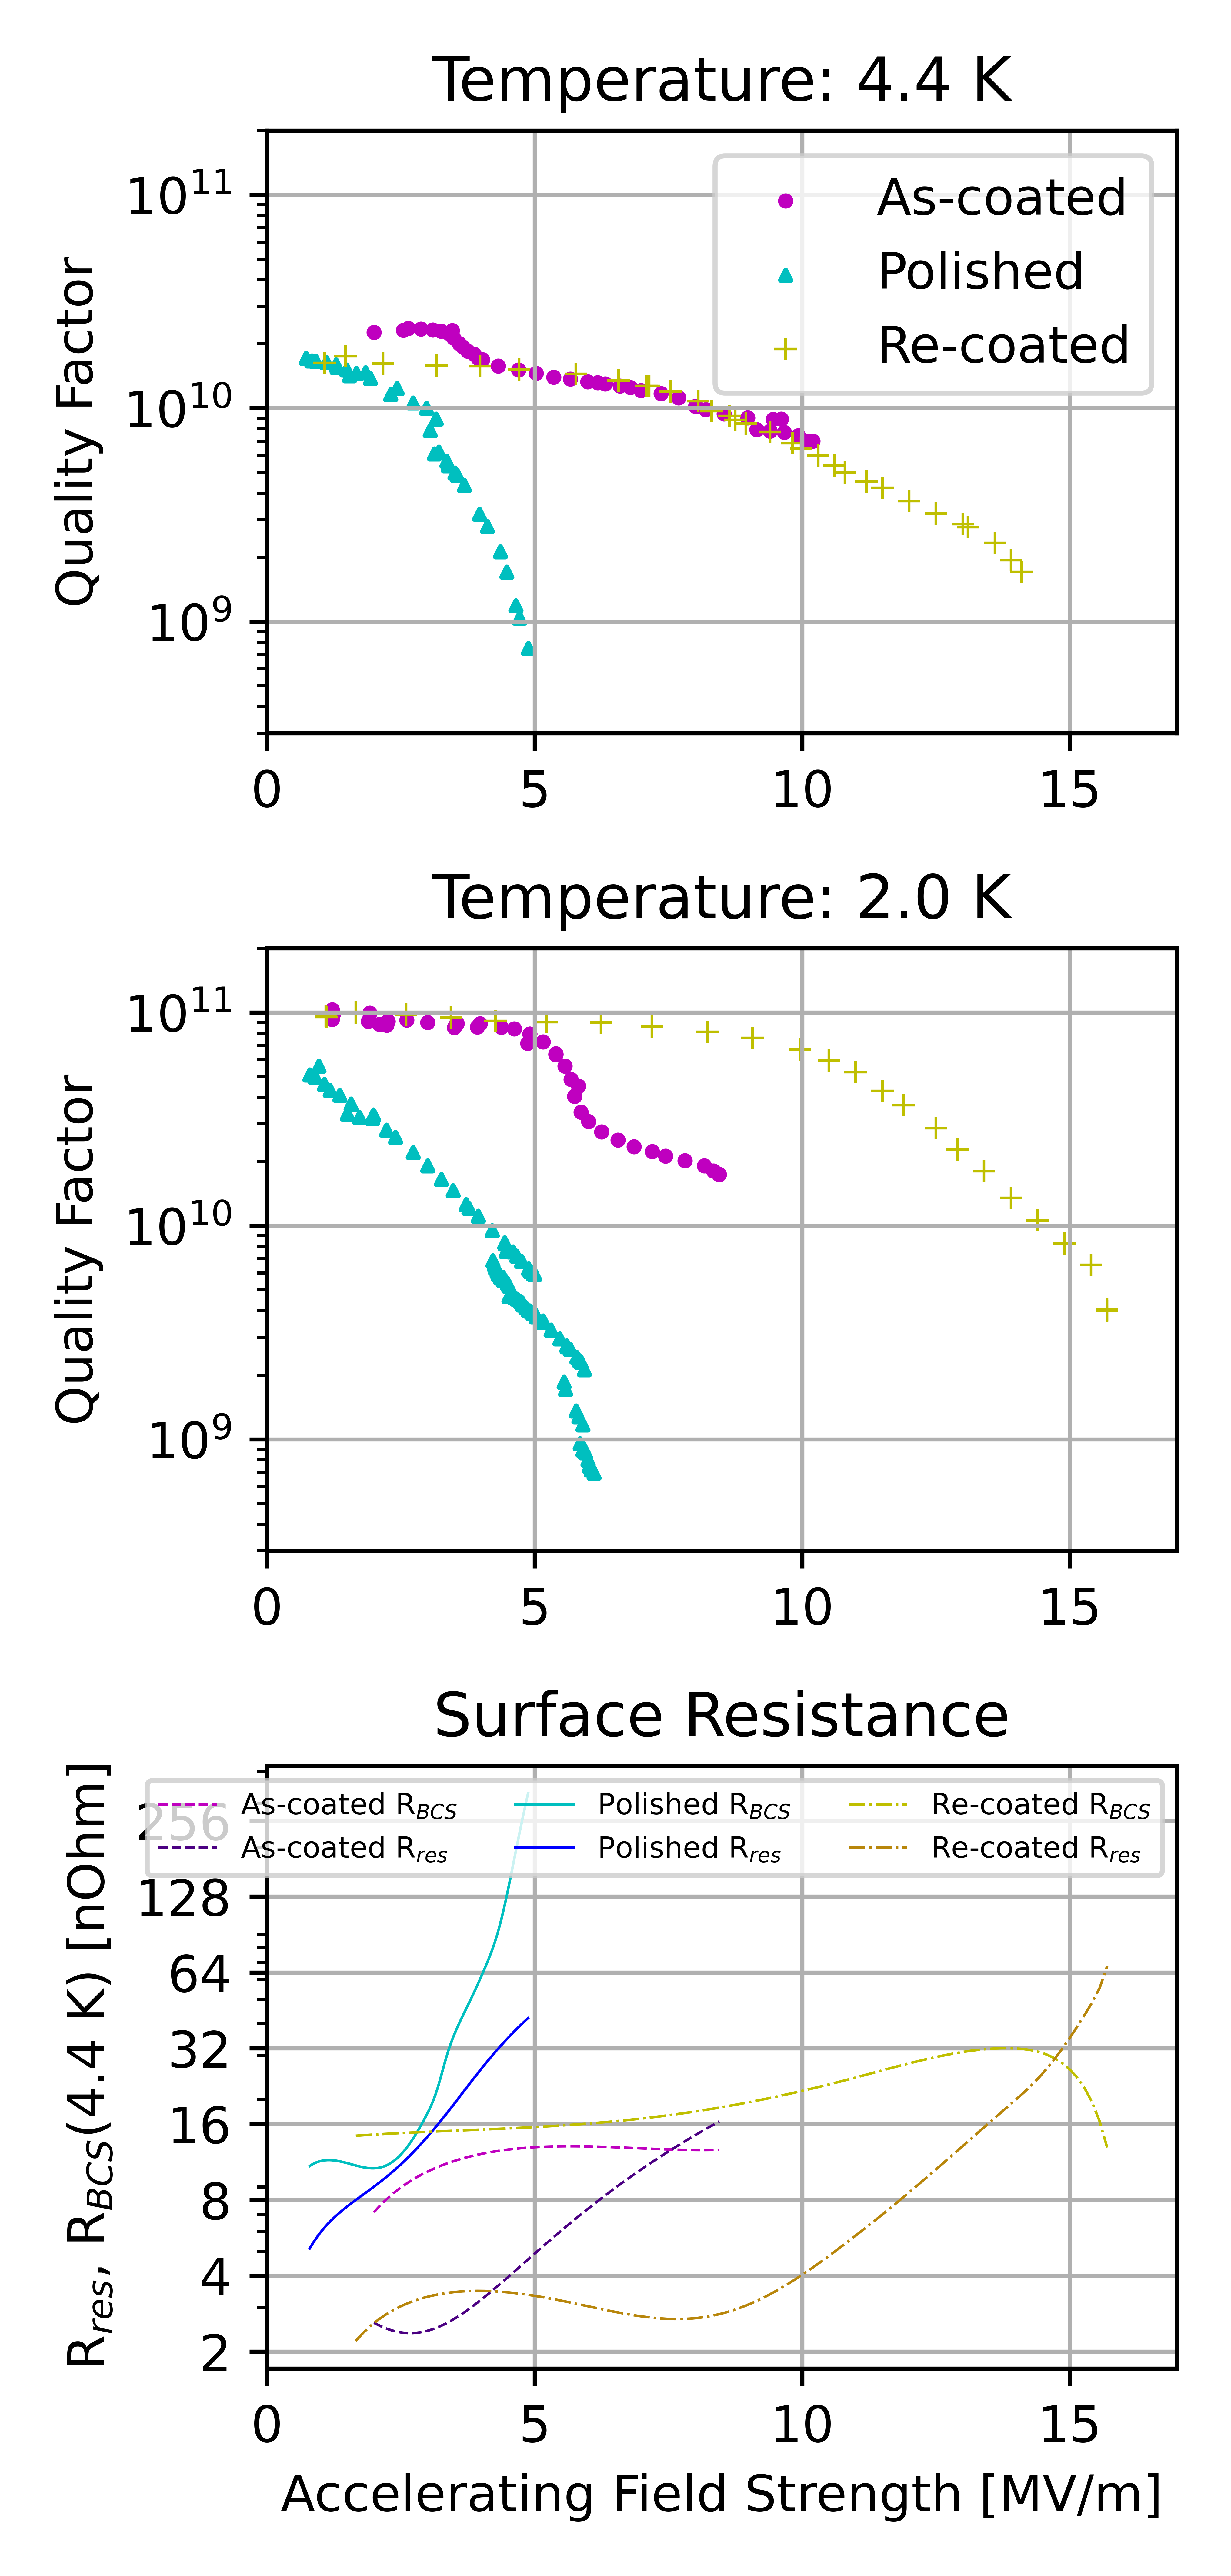
\includegraphics[width=\columnwidth]{../doc/figs/VTS_Test_Graph.png}%
                                \caption{\label{fig:vtstestgraph}The RF performance of the Nb\textsubscript{3}Sn-coated SRF cavity before and after mechanically polished and after a re-coating treatment.}
                            \end{figure}
                        \end{column}
                        \begin{column}{0.5\columnwidth}
                            A Nb\textsubscript{3}Sn-coated single-cell 1.3~GHz cavity was polished for 4~hours followed by high-pressure water rinsing and ultrasonic cleaning for 30~minutes to remove any residual abrasive material. A conservative polishing time was used to minimize the possibility of removing the Nb\textsubscript{3}Sn film while still providing a considerable improvement in surface roughness.
                        \end{column}
                    \end{columns}   
                    \begin{itemize}
                        \item The resulting cavity surface had a mirror-like appearance.
                        \item The as-coated performance was poor, with a maximum gradient of around 10~MV/m and Q of 10\textsuperscript{10} at 4.4~K.
                        \item After polishing, the cavity exhited Q-slope and the maximum gradient was only 5~MV/m.
                        \item A re-coating procedure was applied to repair surface damage and subsurface defects at 1,000~°C, using one third of the normal amount of tin and no SnCl\textsubscript{2}.
                        \item After the re-coating procedure, the Q-slope was ameliorated, and the maximum accelerating gradient increased to 15~MV/m.
                        \item The quality factor of the cavity was also improved over the as-coated state at 2.0~K, but not at 4.4~K.
                    \end{itemize} 
                \end{block}
                \begin{block}{\label{sec:bibliography}Bibliography}
                    \small
                    \bibliographystyle{plain}
                    \bibliography{\jobname}
                \end{block}
                \begin{block}{\label{sec:acknowledgements}Acknowledgements}
                    This manuscript has been authored by Fermi Research Alliance, LLC under Contract No. DE-AC02-07CH11359 with the U.S. Department of Energy, Office of Science, Office of High Energy Physics.
                \end{block}
            \end{column}
        \end{columns}
    \end{frame}
\end{document}